\documentclass[../../master-handout.tex]{subfiles}

\begin{document}

\section{Lecture 2 (Thu, May 14)}
\marginnote{\textbf{Scribes:} Oliver Tattersall (OliverTattersall) \& Owen Waldron (owaldron) \\ \textbf{Date:} Thu, May 14, 2026}

\subsection{Serial Manipulators}

\smallcaps{Serial Manipulators} are kinematic chains of rigid bodies (links) connected by joints.

Rigid Bodies are non-deformable. 
The joints can be connected in two ways, \smallcaps{Revolute} and \smallcaps{Prismatic}. They both have only 1 degree of freedom. Revolute is a rotation around one access like a hinge. Prismatic is a piston, the links push out in translation like a pen ejecting. 

\begin{center}
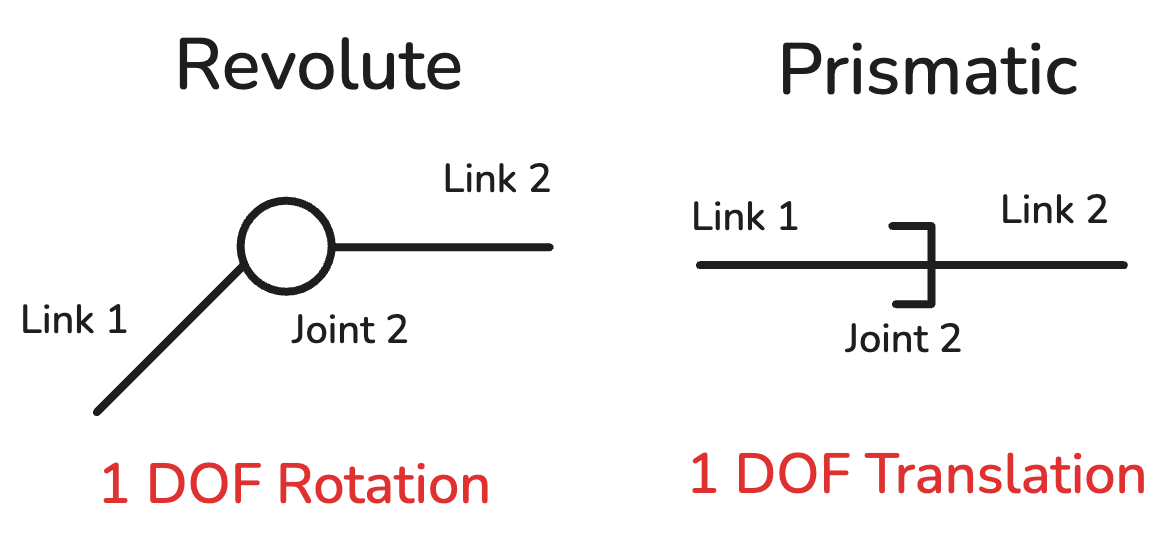
\includegraphics[width=0.7\textwidth]{lecture-2-images/joint_type.png}
\end{center}

A simple manipulator that uses Revolute joints is the \smallcaps{RR Planar Manipulator}. This has 2 revolute joints and two links, as shown below:

\begin{center}
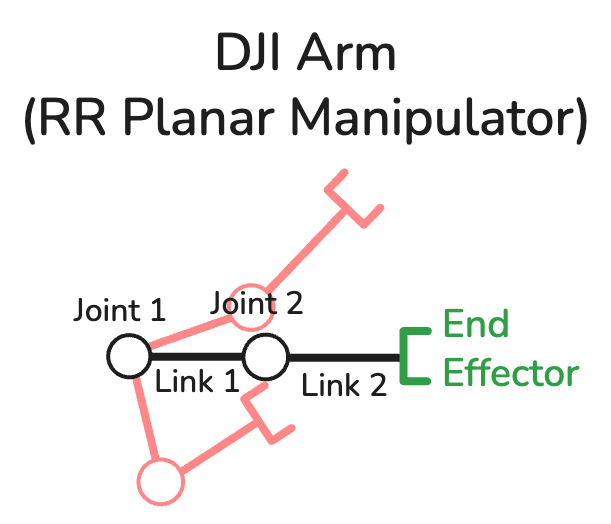
\includegraphics[width=0.7\textwidth]{lecture-2-images/rr_planar.png}
\end{center}

A simple manipulator that uses Prismatic joints is the \smallcaps{3D Cartesian Manipulator}. This has 3 prismatic joints that move along each axis, as shown below. A real world example is a 3D printer, where the location of the nozzle is controlled by 3 prismatic joints to allow placement anywhere in the 3D space.

\begin{center}
\begin{minipage}{0.48\textwidth}
\centering
\includegraphics[width=\linewidth]{lecture-2-images/3d_cart.png}
\end{minipage}\hfill
\begin{minipage}{0.48\textwidth}
\centering
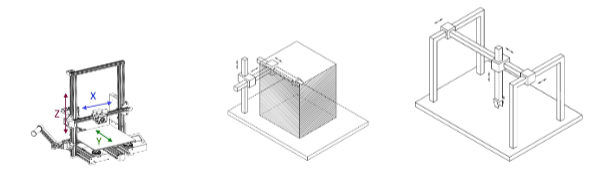
\includegraphics[width=\linewidth]{lecture-2-images/3d_cart_model.png}
\end{minipage}
\end{center}



When we think about joints like the wrist, we can think of them as a composition of 3 back to back revolute joints instead of the more complex spherical joint. This way we can define and recreate its motion much more easily. 
\begin{center}
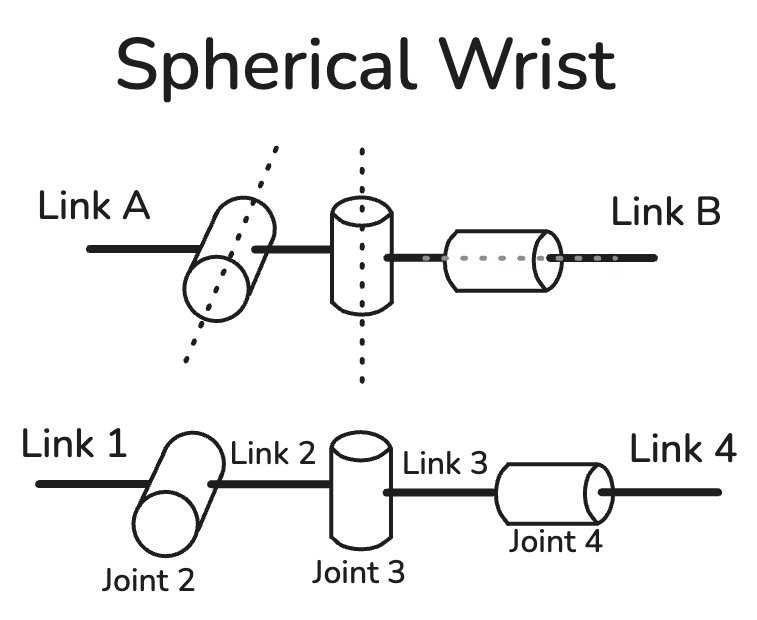
\includegraphics[width=0.7\textwidth]{lecture-2-images/wrist.png}
\end{center}

\smallcaps{SCARA(Selective compliance Assembly Robot Arm)}
From base it has a revolute joint vertically(like your hips rotating), then a resolute join vertically(like holding your arm up with your hand flat down and bending your elbow), then a prismatic joint vertically(like something ejecting from your hands).

\begin{center}
\begin{minipage}{0.48\textwidth}
\centering
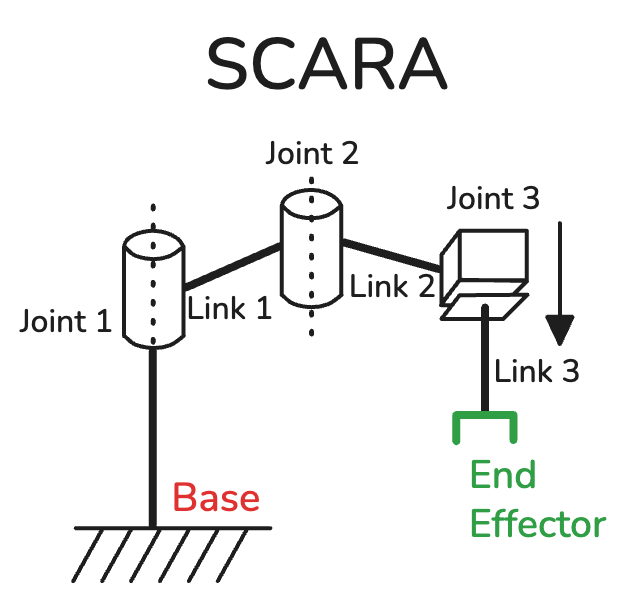
\includegraphics[width=\linewidth]{lecture-2-images/SCARA.png}
\end{minipage}\hfill
\begin{minipage}{0.48\textwidth}
\centering
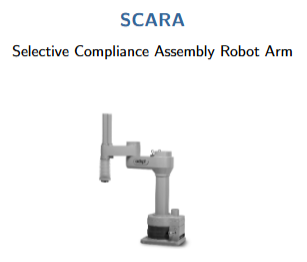
\includegraphics[width=\linewidth]{lecture-2-images/scara_model.png}
\end{minipage}
\end{center}

This is called selective compliant because you can move it in easily in the x-y plane(flat) as the only thing resisting motion is the motors, but the structure of the joints refuses to move in the z direction(up-down). 
\textbf{Note: }There will be a question on selective compliance in either the homework or final.

\begin{center}
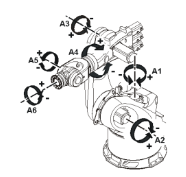
\includegraphics[width=0.5\textwidth]{lecture-2-images/6dof_model.png}
\end{center}
\marginnote{This is an example of a 6-DOF Manipulator}

Gimbal Lock(will be HW1 question)
- When we look at A4 and A6, we can see that they are both rotating around the same axis when A5 is 0. This is called gimbal lock. When A5 is non-zero, there is a distinct solution to the direction. 


The human arm is a 7-DOF manipulator. 7 is special because it is one more than 6 and 6 DOF allows you to access anywhere in space in one unique way, while 7 gives you infinitely many solutions to reach the same location, allow more choice. 


Another example we looked at was Justin, which is a larger humanoid robot with a 4 wheel base. While model-able, quite complex as there are many joints. 


Our end goal is to get our end link to a location to do an action. This last link is the \smallcaps{End Effector}, The point we care about on the link depends on the type of end link. For a camera, we care about where the lens is. For a suction cup on a link, we care about the cup itself. 

\subsection{Parallel Manipulators}
Links and joints that don't necessarily affect one another, but can work together to complete tasks. \smallcaps{Parallel Manipulators} have multiple links and joints that work together to complete tasks while their motion remain independent.
As such, they tend to be very fast and strong, as they have fewer long chains of joints which are brittle. 

\begin{center}
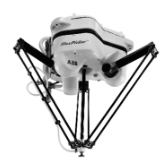
\includegraphics[width=0.4\textwidth]{lecture-2-images/pancake.png}
\end{center}

The \smallcaps{Stewart Platform} has 6 pillars balancing a platform and changing its elevation.
The 6 parallel pillars allow moving very heavy objects very easily, while trying to do so with a high DOF serial manipulator would require exceptional amounts of torque. However, the range of motions of this can be seriously limited in comparison with serial manipulators. 

\begin{center}
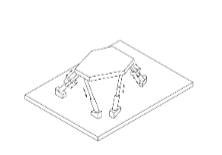
\includegraphics[width=0.5\textwidth]{lecture-2-images/stewart.png}
\end{center}

We will largely use serial manipulators in this course. 

\subsection{Modeling with Math}

Our box model is a manipulator that takes in torques for each joint and outputs the end effector pose.
The End Effector Pose are the 6 digits for orientation and position.
Each joint affects the Pose of the next joints. 

\textbf{Q}: Compute EE Pose as a function of join angles. \smallcaps{Direct Kinematics} answers this question. We will use the relative reference frames to build up the solution. 

\end{document}
